
\chapter{Programming}
\label{app:prog}

In this appendix, I briefly present the code I developed during this internship.
The program was done in \ttt{C++}. As object-oriented programming is extensively used, rather than giving the code detailed working scheme, I will sum up its class structure. The entire code source is available here: \url{https://github.com/Yukee/flume/tree/3D/KT_solver}. 

\section {Containers}

Numerical data and equations are stored in objects called \textit{containers}.

\subsection{Scalar fields}

\begin{figure}[htp]
\centering
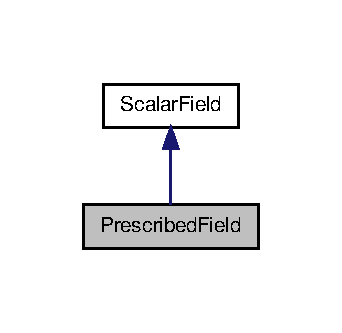
\includegraphics[scale=1.00]{appendix/class_prescribed_field__inherit__graph.pdf}
\caption{}
\label{}
\end{figure}

Numerical data is stored in objects of the \ttt{PrescribedField} class. This class derives from the \ttt{ScalarField} class. 
A \ttt{ScalarField} object represents a scalar field sampled on a discrete grid.
Two such object can be added, multiplied the same way scalar fields can. 
\ttt{ScalarField} are used for example to store the concentration, $\phi$, sampled on the integration grid.
\ttt{PrescribedField} objects are derived from \ttt{ScalarField}. In addition to behaving as scalar fields, \ttt{PrescribedField} objects can store informations about the boundary conditions at the surface bounding the domain of definition of the scalar field.
 One can \textit{prescribe} the value of the field (Dirichlet boundary condition) or the value of its derivative normal to the surface (Von Neumann boundary condition).
 
For testing purposes, I also used \ttt{PeriodicField} objects, behaving like scalar fields with periodic boundary conditions.

\subsection{Flux functions}

\begin{figure}[htp]
\centering
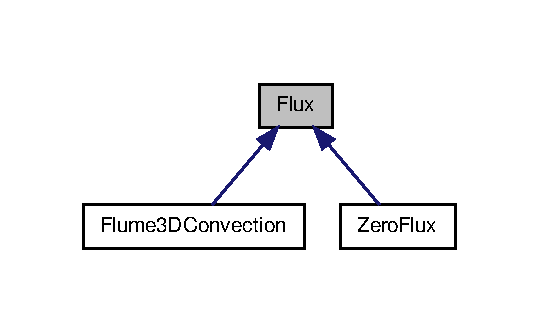
\includegraphics[scale=1.00]{appendix/class_flux__inherit__graph.pdf}
\caption{}
\label{flux}
\end{figure}

\ttt{Flux} objects behave like functions. They are used to store the information about what is the flux function $f$ (cf appendix \ref{app:finite} for the definition) in the conservation law we want to solve.
If we want to construct a new flux function, we just have to derive the base class (figure \ref{flux}).

\subsection{Equations}

\ttt{Equation} objects are used to store informations about the equation we want to solve numerically, namely
\begin{equation}
	\p{}{t} \phi + \p{}{x} f(\phi, x) = \p{}{x} D \left( \phi, \p{\phi}{x} \right) + S(\phi, x)
\end{equation}

An \ttt{Equation} stores the form of the advection flux $f$, of the diffusion flux $D$ and of the source term $S$ in \ttt{Flux} objects.

Note that this equation is slightly different from a conservation law, because of the addition of the source term $S$ and the diffusion term $D$, but it can be solved in the same way. 
A source term appear for example when we solve the 2D segregation equation in the centre plane, as explained in chapter 2. 
A diffusion flux will appear if we wish to model the effect of viscosity on the granular flow. It was not used during the internship, but can be handled by the program, and may be used in the future.

\section{Solvers}

\begin{figure}[htp]
\centering
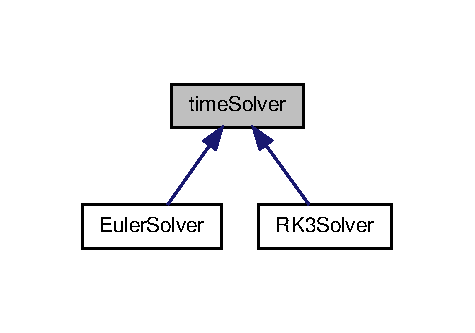
\includegraphics[scale=1.00]{appendix/classtime_solver__inherit__graph.pdf}
\caption{}
\label{}
\end{figure}

Solvers are objects designed to integrate the above equation. 
To do the time evolution, the \ttt{timeSolver} calls repetitively the \ttt{KTSolver}, whose role is to compute the numerical fluxes at the edges of the cells (cf appendix \ref{app:finite}).

For time stepping, we used the simple Euler method, and the more sophisticated order three Runge-Kutta method. 
If we want to construct a new method, we just have to derive the \ttt{timeSolver} class.

I would like to insist on the fact that the program is very general. It is able to solve any system of laws of the type (1.1), in any number of spatial dimensions.

\section{Another approach}
At the end of my internship, I created a new code based on a totally different approach. 
The base container of this new code was the \ttt{Cell}. A \ttt{Cell} object represent a finite volume cell (cf appendix ??). It contains the value of the solved field, and the values of the numerical fluxes at its edges.
A \ttt{CellArray} object stores the cells forming the integration domain. 

This approach is powerful, especially for handling boundary conditions. for example, if we want to prescribe the flux to be zero at the boundary of the domain, we just have to create a new class \ttt{BoundaryCell} derived from \ttt{Cell}, and taking into account this specificity. The \ttt{CellArray} object will then contain an heterogeneous collection of \ttt{Cell} objects (forming the inner part of the integration domain) and \ttt{BoundaryCell} objects (forming the boundary of the integration domain).

Using this approach, it is also very easy to use different numerical schemes to integrate the differential equation. I was thus able to test a number of different approaches. The source code is available here: \url{https://github.com/Yukee/finite-volume/tree/master/KT_new_1D}.
